
\documentclass[12pt]{article} 
\usepackage{alphalph}
\usepackage[utf8]{inputenc}
\usepackage[russian,english]{babel}
\usepackage{titling}
\usepackage{amsmath}
\usepackage{graphicx}
\usepackage{enumitem}
\usepackage{amssymb}
\usepackage[super]{nth}
\usepackage{everysel}
\usepackage{ragged2e}
\usepackage{geometry}
\geometry{top=1.0in,bottom=1.0in,left=1.0in,right=1.0in}
\newcommand{\subtitle}[1]{%
  \posttitle{%
    \par\end{center}
    \begin{center}\large#1\end{center}
    \vskip0.5em}%

}
\usepackage{hyperref}
\hypersetup{
colorlinks=true,
linkcolor=blue,
filecolor=magenta,      
urlcolor=blue,
citecolor=blue,
}

\urlstyle{same}
\renewcommand*\familydefault{\ttdefault}
\EverySelectfont{%
\fontdimen2\font=0.4em% interword space
\fontdimen3\font=0.2em% interword stretch
\fontdimen4\font=0.1em% interword shrink
\fontdimen7\font=0.1em% extra space
\hyphenchar\font=`\-% to allow hyphenation
}

\begin{document}

%------------------------------------------------------------------------------------------
% Title
%------------------------------------------------------------------------------------------

\author{Name: }
\title{Final Review Packet\\European History AP}
\subtitle{1347 $-$ Present}
\date{Date: }
\maketitle
\begin{center}
    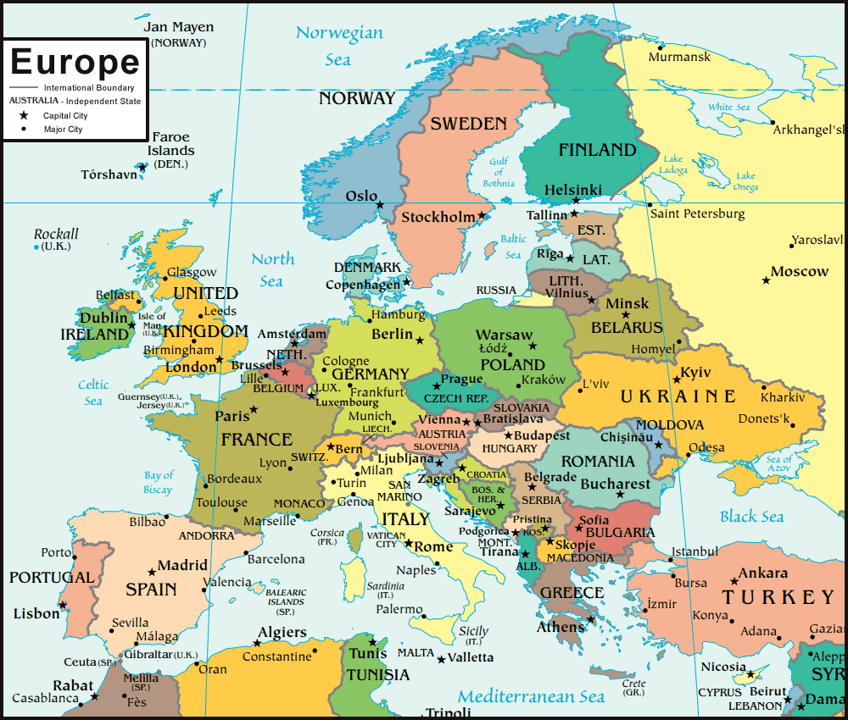
\includegraphics[width=\textwidth]{Europa.png}
\end{center}
\newpage
\tableofcontents
\newpage

%------------------------------------------------------------------------------------------
% Questions
%------------------------------------------------------------------------------------------



\begin{center}
\section{\underline{Renaissance}}
\end{center}

\begin{enumerate}[label=]
\subsection{Causes}
\item
\end{enumerate}
\vspace{-35pt}
\begin{enumerate}

\item Philosophical/Religious $-$ 
    
\item Political (city states) $-$ 

\item Economic $-$ 

\item Social $-$ 

\subsection{Terms}

\item Humanism $-$ 

\item Individualism $-$ 

\item Secularism $-$ 

\subsection{People}

\item Machiavelli $-$ 

\item Christine de Pisan $-$ 

\item Valla $-$ 

\item Petrarch $-$ 

\item Dante $-$ 

\item Boccaccio $-$ 

\item Medici Family $-$ 

\item Da Vinci $-$ 

\item Michelangelo $-$ 

\item Raphael $-$ 

\item Alexander VI $-$ 

\item Julius II $-$ 

\item Leo X $-$ 

\subsection{Northern Renaissance}

\item Erasmus $-$ 

\item More $-$

\item Durer $-$ 

\item Printing Press $-$ 

\subsection{Compare and Contrast the Italian and Northern Renaissances}

\item Similarities $-$ 

\item Differences $-$ 

\subsection{Effects}

\item Philosophical/Religious $-$ 

\item Political $-$ 

\item Economic $-$ 

\item Social $-$ 

\item Education $-$ 

\begin{center}
\section{\underline{The New Monarchs}}
\end{center}

\subsection{Causes}

\item Political $-$ 

\item Economic $-$ 

\item Need for Permanent Standing Army $-$

\item Taxation to Pay For Army and Bureaucracy $-$ 

\item Classes
\begin{enumerate}[label=\arabic{*}.]
\setcounter{enumii}{36}
\item Nobles $-$

\item Church $-$

\item Middle $-$

\end{enumerate}

\subsection{Political Situation $-$ 16\textsuperscript{th} Century}

\setcounter{enumi}{39}

\item Spain $-$

\item France $-$

\item England $-$

\item Holy Roman Empire $-$

\subsection{Spain \& The Holy Roman Empire}

\item Ferdinand \& Isabella $-$

\item Charles V $-$

\item Phillip II $-$

\subsection{England}

\item Henry VII $-$

\item Henry VIII $-$

\item Elizabeth I $-$

\begin{center}
\section{\underline{The Age of Exploration}}
\end{center}

\subsection{Causes}

\item Political $-$

\item Economic $-$

\item Technological $-$

\item Religious $-$

\subsection{People}

\item Prince Henry the Navigator $-$

\item Columbus $-$

\item Magellan $-$

\item Diaz $-$

\item Da Gama $-$

\item Cortes $-$

\item Pizzaro $-$

\subsection{Effect on the Americas}

\item Destruction of Civilizations $-$

\item African Slavery $-$

\subsection{Effect on Europe} $-$

\item Intellectual $-$

\item Economic $-$

\item Political $-$

\subsection{Colombian Exchange} 

\item Diseases $-$ 

\item Food $-$ 

\begin{enumerate}[label=\arabic{*}.]
\setcounter{enumii}{67}
\item Potato on Population of Northern Europe $-$ 
\end{enumerate}
\setcounter{enumi}{68}
\item Price Revolution (Inflation) $-$

\begin{enumerate}[label=\arabic{*}.]
\setcounter{enumii}{69}
\item Causes $-$

\item Effects $-$
\end{enumerate}
\setcounter{enumi}{71}
\section{\underline{Religious Reformation}}

\subsection{Causes}

\item Religious $-$

\item Political $-$

\item Economic $-$

\item Social $-$

\item Northern European Renaissance Humanism $-$ 

\item Reason's for Luther's Success $-$ 

\subsection{Effects}

\item Religious $-$ 

\item Political $-$ 

\item Economic $-$ 

\item Social $-$ 

\subsection{Important People}

\item Wycliffe $-$ 

\item Huss $-$ 

\item Luther $-$ 

\item Zwingli $-$ 

\item Calvin $-$ 

\item Henry VIII $-$ 

\item Edward VI $-$ 

\item Bloody Mary $-$ 

\item Elizabeth I $-$ 

\item Mary, Queen of Scots $-$

\item Leo X $-$ 

\item Tetzel $-$ 

\item Frederick, Duke of Saxony $-$ 

\item Charles V $-$

\item Phillip II $-$

\item Ignatius Loyola $-$

\subsection{Terms}

\item Simony $-$

\item Nepotism $-$

\item Indulgences $-$

\item Babylonian Captivity $-$

\item Great Schism $-$ 

\item Protestant $-$

\item Antibaptist $-$

\item Salvation by Faith Alone $-$

\item Sole Authority of the Bible $-$

\item Sacraments $-$

\item Diet of Worms $-$ 

\item Peasant's Revolt $-$

\item Predestination $-$ 

\item Protestant Work Ethic $-$ 

\item Catholic/Counter Reformation $-$ 

\begin{enumerate}[label=\arabic{*}.]
\setcounter{enumii}{112}
\item Affirmation of Doctrines $-$

\item Reforms of Abuses $-$

\end{enumerate}
\setcounter{enumi}{114}
\item Council of Trent $-$

\item Jesuits $-$  

\item Baroque Art $-$

\item Church State Relations (Luther vs. Calvin) $-$

\item Six Articles $-$

\item Peace of Augsburg (1555) $-$

\section{\underline{Religious Wars}}

\subsection{Dutch Revolt (1508 $-$ 1609)}

\subsubsection{Causes}

\item Political $-$ 

\item Economic $-$ 

\item Religious $-$ 

\subsubsection{People}

\item Philip II

\item Duke of Alva

\item Elizabeth I (Spanish Armada)

\subsubsection{Effects}

\subsection{French Civil War (1562 $-$ 1598)}

\subsubsection{Causes}

\item Political $-$ 

\item Economic $-$

\item Religious $-$ 

\subsubsection{People}

\item Catherine de Medici $-$

\item Henry IV of Navarre $-$ 

\item Huguenots $-$ 

\item St. Bartholomew's Day Massacre $-$

\item Edict of Nantes $-$ 

\item Politique $-$ 

\subsubsection{Effects}

\subsection{Thirty Year's War (1618 $-$ 1648)}

\subsubsection{Causes}

\item Political $-$ 

\item Economic $-$ 

\item Religious $-$ 

\item Limits of Peace of Augsberg (1555) $-$

\subsubsection{The War}

\item Habsburgs vs. Most of Europe $-$

\item Phases

\begin{enumerate}[label=\arabic{*}.]
\setcounter{enumii}{141}

\item Bohemian (Bad) $-$

\item Danish (Danish Eat) $-$ 

\item Swedish (Swedish) $-$ 

\item French-Swedish (Fish) $-$

\end{enumerate}
\setcounter{enumi}{145}
\item Role of France $-$ 

\item Defenestration of Prague $-$ 

\item Wallenstein $-$ 

\item Gustavus Adolphus $-$ 

\item Richelieu $-$ 

\item Results (Peace of Westphalia) $-$  

\section{\underline{Constitutionalism}}

\subsection{Tudors}

\item Henry VII $-$ 

\item Henry VIII $-$ 

\item Edward VI $-$ 

\item Mary I (Bloody Mary) $-$ 

\item Elizabeth I $-$ 

\subsection{Stuarts}

\item James I $-$ 

\item Charles I $-$ 

\item Charles II $-$

\item James II $-$ 

\item William III \& Mary II $-$

\item Anne $-$ 

\item Cromwell $-$ 

\subsection{Documents}

\item Magna Carta $-$ 

\item Petition of Right $-$ 

\item Habeas Corpus $-$ 

\item Bill of Right $-$ 

\subsection{English Civil War (1640 $-$ 1649)}

\item Causes $-$ 

\item Reasons for Puritans Winning $-$ 

\item Effects $-$

\subsection{Glorious Revolution (1688)}

\item Causes $-$

\item Effects $-$

\subsection{Terms}

\item Church of England $\rightarrow$ Anglican Church $-$

\item Puritans $-$ 

\item Cavaliers $-$ 

\item Roundheads $-$ 

\item New Model Army $-$ 

\item Commonwealth $-$ 

\item Rump Parliament $-$ 

\item Levellers $-$ 

\item Restoration $-$ 

\item Test Act $-$ 

\item Whigs $-$ 

\item Tories $-$ 

\section{\underline{Absolutism}}

\item Causes $-$ 

\subsection{French Monarchs, Ministers, and Policies}

\item Henry IV $-$

\begin{enumerate}[label=\arabic{*}.]
\setcounter{enumii}{186}

\item Edict of Nantes $-$ 

\item Duke of Sully $-$

\end{enumerate} 
\setcounter{enumi}{188}

\item Louis XIII $-$

\begin{enumerate}[label=\arabic{*}.]
\setcounter{enumii}{189}

\item Cardinal Richelieu $-$ 

\end{enumerate}
\setcounter{enumi}{190}

\item Louis XIV (The Sun King) $-$

\begin{enumerate}[label=\arabic{*}.]
\setcounter{enumii}{191}
\item L'\'etat, C'est Moi $-$

\item Cardinal Mazarin $-$ 

\item Fronde $-$ 

\item Versailles $-$

\begin{enumerate}[label=\arabic{*}.]
\setcounter{enumiii}{195}

\item Purpose/Goal $-$

\item Effect $-$

\end{enumerate}
\setcounter{enumii}{197}

\item Bishop Bossuet (Divine Right) $-$

\item Colbert $-$ 

\item Mercantilism $-$ 

\item Revocation of Edict of Nantes $-$ 

\item Foreign Policy Goals $-$ 

\end{enumerate}

\subsection{Wars}
\setcounter{enumi}{202}

\item Dutch Wars $-$

\item War of Spanish Succession $-$

\item Cost $-$ 

\item Accomplishment $-$ 

\item Peace of Utrecht $-$ 

\item Balance of Power $-$ 

\item Legacy $-$ 

\item Culture \& Arts $-$ 

\item Finances \& Taxation $-$ 

\item Economic Development $-$ 

\item Louis XV $-$ 

\begin{enumerate}[label=\arabic{*}.]
\setcounter{enumii}{213}
 
\item Cardinal Fleury $-$ 

\end{enumerate}
\setcounter{enumi}{214}

\section{\underline{Scientific Revolution \& The Enlightenment}}

\item Pre-Renaissance Science $-$ 

\begin{enumerate}[label=\arabic{*}.]
\setcounter{enumii}{215}

\item Purpose $-$ 

\item Method $-$

\end{enumerate}
\setcounter{enumi}{217}

\item View of Universe $-$ 

\begin{enumerate}[label=\arabic{*}.]
\setcounter{enumii}{218}

\item Aristotle \& Ptolemy $-$ 

\item Copernicus \& Heliocentric Theory $-$ 

\item Brahe Contribution $-$ 

\item Kepler's Contribution $-$ 

\item Galileo's Contributions $-$ 

\begin{enumerate}[label=\arabic{*}.]
\setcounter{enumiii}{223}

\item Experimentation $-$ 

\item Telescope $-$


\end{enumerate}



\end{enumerate}
\setcounter{enumi}{225}

\subsection{Persecution by the Roman Catholic Church}

\item Effect on Science in Catholic Countries $-$

 
\begin{enumerate}[label=\arabic{*}.]
\setcounter{enumii}{226}

\item Newton $-$ 

\begin{enumerate}[label=\arabic{*}.]
\setcounter{enumiii}{227}

\item Law of Universal Gravitation $-$ 

\item \textit{Principia} $-$

\end{enumerate}
\setcounter{enumii}{229}

\item Bacon $-$ 

\begin{enumerate}[label=\arabic{*}.]
\setcounter{enumiii}{230}

\item Inductive Reasoning $-$ 

\item Method $-$

\item Empiricism $-$

\end{enumerate}
\setcounter{enumii}{233}

\item Descartes $-$ 

\begin{enumerate}[label=\arabic{*}.]
\setcounter{enumiii}{234}

\item Deductive Reasoning $-$ 

\item Cartesian Dualism $-$

\item "Cognito ergo su" $-$ 

\end{enumerate}

\end{enumerate}
\setcounter{enumi}{237}

\item Products of Scientific Revolution $-$

\begin{enumerate}[label=\arabic{*}.]
\setcounter{enumii}{238}

\item Intellectual $-$ 

\item Emergence of Scientific Community $-$

\item Scientific Method $-$ 

\item Belief in Reason $-$

\item Influence on Enlightenment $-$

\end{enumerate}
\setcounter{enumi}{243}
\subsection{Enlightenment}

\subsubsection{Important People}

\item Hobbes $-$ 

\begin{enumerate}[label=\arabic{*}.]
\setcounter{enumii}{244}

\item Human Nature $-$ 

\item Government $-$

\end{enumerate}
\setcounter{enumi}{246}

\item Locke $-$ 

\begin{enumerate}[label=\arabic{*}.]
\setcounter{enumii}{247}

\item Human Nature $-$ 

\item Government $-$

\end{enumerate}
\setcounter{enumi}{249}
\subsubsection{Philosophes}

\item Salons $-$ 

\item Elite vs. Masses $-$

\item Montesquieu $-$ 

\begin{enumerate}[label=\arabic{*}.]
\setcounter{enumii}{252}

\item \textit{Spirit of the Laws} $-$

\end{enumerate}
\setcounter{enumi}{253}

\item Voltaire $-$ 

\begin{enumerate}[label=\arabic{*}.]
\setcounter{enumii}{254}

\item Deism $-$ 

\item \textit{Treatise on Toleration} $-$

\item \textit{Candide} $-$ 

\item Admiration for Britain $-$ 

\item Frederick the Great $-$

\end{enumerate}
\setcounter{enumi}{259}

\item Rousseau $-$ 

\begin{enumerate}[label=\arabic{*}.]
\setcounter{enumii}{260}

\item Influence on Romantic Movement $-$ 

\item Effects of Civilization $-$

\item \textit{Social Contract} $-$

\begin{enumerate}[label=\arabic{*}.]
\setcounter{enumiii}{263}

\item General Will \& Totalitarianism $-$

\end{enumerate}
\setcounter{enumii}{264}

\item \textit{Emile}

\begin{enumerate}[label=\arabic{*}.]
\setcounter{enumiii}{265}

\item Education $-$ 

\item Treatment of Children $-$

\end{enumerate}
\end{enumerate}
\setcounter{enumi}{267}

\item Diderot $-$ 

\begin{enumerate}[label=\arabic{*}.]
\setcounter{enumii}{268}

\item \textit{Encyclop\'edie} $-$ 

\end{enumerate}
\setcounter{enumi}{269}

\item Physiocrates $-$

\begin{enumerate}[label=\arabic{*}.]
\setcounter{enumii}{270}

\item Quesnay $-$ 

\begin{enumerate}[label=\arabic{*}.]
\setcounter{enumiii}{271}

\item Laissez-faire $-$ 

\end{enumerate}
\setcounter{enumii}{272}

\item Adam Smith $-$

\begin{enumerate}[label=\arabic{*}.]
\setcounter{enumiii}{273}

\item \textit{Wealth of Nations} $-$ 

\item Capitalism $-$

\end{enumerate}

\end{enumerate}
\setcounter{enumi}{275}

\subsection{Enlightened Despotism}

\item Characteristics $-$

\begin{enumerate}[label=\arabic{*}.]
\setcounter{enumii}{276}

\item Reform of Justice and Legal Systems $-$ 

\item Improve Society \& Promote Happiness $-$

\item Religious Toleration $-$

\item Freedom of Press, etc. $-$ 

\item Economic Reform $-$ 

\item Education Reform $-$ 

\item Improve Efficiency $-$ 


\end{enumerate}
\setcounter{enumi}{283}

\item Truce Goal $-$

\subsection{Enlightened Monarchs}

\item Frederick the Great (Prussia) $-$ 

\item Peter the Great (Russia) $-$

\item Catherine the Great (Russia) $-$ 

\item Maria Theresa (Austria) $-$ 

\item Joseph II (Austria) $-$


\section{\underline{French Revolution}} 

\item \begin{tabular}{l c c c c}

Old Regime & Occupation & Taxation & Status & Problems/Gripes\\
\hline
1\textsuperscript{st} Estate & & & & \\
\hline
2\textsuperscript{nd} Estate & & & & \\
\hline
3\textsuperscript{rd} Estate & & & & \\
\hline
Bourgeoisie & & & & \\
\hline
Sans Culottes & & & & \\
\hline
Peasants & & & & \\
\hline

\end{tabular}

\subsection{Causes}

\item Finances $-$

\begin{enumerate}[label=\arabic{*}.]
\setcounter{enumii}{291}

\item Wars $-$

\item Versailles $-$

\item Interest on Debt $-$ 

\end{enumerate}
\setcounter{enumi}{294}

\item Inadequate Taxation $-$ 

\begin{enumerate}[label=\arabic{*}.]
\setcounter{enumii}{295}

\item Nobles R\'ecalcitrante $-$

\end{enumerate}
\setcounter{enumi}{296}

\item Injustice $-$

\item Enlightenment $-$ 

\item Louis XVI \& Marie Antoinette $-$

\item Parlement of Paris $-$ 

\item Estates General $-$ 

\item Cahiers de dol\'eances $-$

\item National Assembly $-$

\item Tennis Court Oath $-$ 

\subsection{1\textsuperscript{st} Phase $-$ Moderate Stage (1789 $-$ 1792)}

\item Fall of Bastille $-$ 

\item Great Fear $-$ 

\item Abolition of Feudalism $-$ 

\item Declaration of Rights of Man and Citizen $-$ 

\item Slogan $-$ 

\item Sans-Culottes Women Bring Back Royalty $-$ 

\item Financial $-$ 

\begin{enumerate}[label=\arabic{*}.]
\setcounter{enumii}{311}

\item Seizure of Church Property $-$

\item Assignats $-$ 

\end{enumerate}
\setcounter{enumi}{313}

\item Civil Constitution of Clergy $-$ 

\item Establishment of Departments $-$ 

\item Metric System $-$ 

\item Failure of Royal Family to Escape $-$ 

\item Edmund Burke $-$

\subsection{Reflections on the Revolution in France}

\item \textit{A Vindication of the Rights of Women} (Mary Wollstonecraft) $-$

\item \textit{Declaration of Rights of Women} (Olympe de Gouges) $-$

\subsection{2\textsuperscript{nd} Phase $-$ Radical Stage (1792 $-$ 1795)}

\item National Convention $-$ 

\item Jacobins $-$ 

\item Girondists $-$ 

\item Mountains $-$ 

\item Danton $-$ 

\item Marat $-$ 

\item Robespierre $-$ 

\item Declaration of Republic $-$ 

\item Execution of King and Queen $-$ 

\item Guillotine $-$ 

\item Brunswick Manifesto \& First Coalition $-$ 

\item Nationalism $-$ 

\item Levee en Masse $-$ 

\item Economic Accomodations to Sans Culottes $-$

\item Reign of Terror $-$ 

\item Committee of Public Safety $-$ 

\item Republic of Virtue $-$ 

\subsection{3\textsuperscript{rd} Phase $-$ Reactionary Stage (1795 $-$ 1799)}

\item Directory $-$ 

\item Corruption $-$ 

\subsection{Napoleonic Era (1799 $-$ 1815)}

\item Background $-$ 

\item Military Victories in Italy $-$ 

\item Invasion of Egypt $-$ 

\item Coup d'etat $-$ 

\item Consulate $-$ 

\item Emperor $-$ 

\item Concordat with the Roman Catholic Church $-$ 

\item Napoleonic Code $-$ 

\item Education Reforms $-$ 

\item Financial Reforms $-$ 


\begin{enumerate}[label=\arabic{*}.]
\setcounter{enumii}{349}

\item Bank of France $-$

\end{enumerate}
\setcounter{enumi}{350}

\item Meritocracy $-$ 

\begin{enumerate}[label=\arabic{*}.]
\setcounter{enumii}{351}

\item Legion of Honor $-$ 

\end{enumerate}
\setcounter{enumi}{352}

\item Conquest of Europe $-$ 

\item Failure of Trafalgar $-$ 

\item Foreign Policy \& Military Mistakes $-$ 

\begin{enumerate}[label=\arabic{*}.]
\setcounter{enumii}{355}

\item Continental System $-$

\item Peninsular (Spanish) War $-$

\item Invasion of Russia $-$ 

\end{enumerate}
\setcounter{enumi}{358}

\item Defeat at Battle of Nations $-$ 

\item Exile to Elba $-$ 

\item Escape from Elba \& 100 Days $-$ 

\item Battle of Waterloo \& Exile to St. Helena $-$ 

\section[\underline{Mercantilism, Agricultural Revolution, \& Industrial Revolution}]{\underline{Mercantilism and the Industrial Revolution}}

\item Mercantilism $-$ 

\subsection{Agriculture}

\item Causes $-$ 

\item Dutch \& English $-$ 
 
\begin{enumerate}[label=\arabic{*}.]
\setcounter{enumii}{365}

\item Reclamation of Land $-$

\end{enumerate}
\setcounter{enumi}{366}

\item Turnip Townshend $-$ 

\begin{enumerate}[label=\arabic{*}.]
\setcounter{enumii}{367}

\item Nitrogen-Fixing Crops $-$

\item Crop Rotation $-$

\end{enumerate}
\setcounter{enumi}{369}

\item New Farm Tools $-$ 

\begin{enumerate}[label=\arabic{*}.]
\setcounter{enumii}{370}

\item Jethro Tull $-$ Seed Drill $-$

\item Iron Plow $-$ 

\end{enumerate}
\setcounter{enumi}{372}

\item Selective Breeding of Animals $-$ 

\begin{enumerate}[label=\arabic{*}.]
\setcounter{enumii}{373}

\item Bakewell $-$

\item Protein Food $-$

\item Manure/Fertilizer $-$ 


\end{enumerate}
\setcounter{enumi}{376}

\item Enclosure Movement $-$ 

\begin{enumerate}[label=\arabic{*}.]
\setcounter{enumii}{377}

\item Effects $-$ 

\end{enumerate}
\setcounter{enumi}{378}

\subsection{Industrial Revolution}

\item Began in England in $-$ 

\item Textile Industry Inventions $-$ 

\item Steam Engine $-$ 

\item Relatively Inexpensive Iron \& Steel $-$

\item Transportation Systems $-$

\begin{enumerate}[label=\arabic{*}.]
\setcounter{enumii}{383}

\item Steam Boats/Ships $-$

\item Railroads $-$ 


\end{enumerate}
\setcounter{enumi}{385}

\item Spread of Industrialization $-$ 

\item Results $-$ 

\item Working Conditions of Proletariat $-$ 

\begin{enumerate}[label=\arabic{*}.]
\setcounter{enumii}{388}

\item Hours \& Wages $-$

\item Women $-$

\item Children $-$ 


\end{enumerate}
\setcounter{enumi}{391}

\item Sadler Committee $-$ 

\item Proletariat $-$ 

\item Change in Family Sturcture $-$ 

\item No Longer Unit of Production $-$ 

\item Just Unit of Consumption $-$ 

\item Relation of Parents to Children $-$ 

\item Urbanization $-$ 

\begin{enumerate}[label=\arabic{*}.]
\setcounter{enumii}{398}

\item Sanitation $-$

\item Crowding $-$

\item Disease $-$ 


\end{enumerate}
\setcounter{enumi}{401}

\item Luddites $-$ 

\item Increased Power of State $-$ 

\item Increased Power of Military $-$ 

\item Military Industrial Complex $-$ 

\item Reaction of Romantics $-$ 

\begin{enumerate}[label=\arabic{*}.]
\setcounter{enumii}{406}

\item Writers $-$ 

\item Composers $-$ 

\item Artists $-$  


\end{enumerate}
\setcounter{enumi}{409}

\subsection{Reaction of Economists}

\item \begin{tabular}{l c c}
\textsc{Classical School} & \textsc{Writings} & \textsc{Main Ideas} \\
\hline
Adam Smith & & \\
\hline
Malthus & & \\
\hline 
Ricardo & & \\
\hline
Benthem & & \\
\hline
John Stuart Mill & & \\
\hline
Saint Simon & & \\
\hline
Owen & & \\
\hline
Blanc & & \\
\hline
Engels & & \\
\hline
Marx & & \\
\end{tabular}

\item Basic Theories $-$

\begin{enumerate}[label=\arabic{*}.]
\setcounter{enumii}{411}

\item Economic View of History $-$

\item Class Struggle $-$

\item Inevitability of Revolution $-$ 

\item Surplus Value $-$

\item Communist Society $-$ 

\end{enumerate}
\setcounter{enumi}{416}

\section{\underline{The Congress of Vienna}}

\item Legitimacy $-$ 

\item Undue Influence of French Revolution $-$ 

\item Concert of Europe/Quadruple Alliance $-$

\item Nationalism $-$

\item Metternich in the Congress of Vienna $-$

\item \begin{tabular}{l c c c}

\hline  
Early 19\textsuperscript{th} Century: & Definition & Goals & Supporters \\
\hline
Conservative & & & \\
\hline
Reactionary & & & \\
\hline
Liberal & & & \\
\hline
Romantic & & & \\
\hline

\end{tabular}

\item German Confederation $-$

\begin{enumerate}[label=\arabic{*}.]
\setcounter{enumii}{423}

\item Carlsbad Decrees $-$

\end{enumerate}
\setcounter{enumi}{424}

\item Greek Revolution \& Independence $-$

\item Belgian Revolution \& Independence $-$

\subsection{Russia}

\item Alexander I $-$ 

\item Decembrists Revolution $-$ 

\item Nicholas I $-$ Reactionary Policies

\begin{enumerate}[label=\arabic{*}.]
\setcounter{enumii}{429}

\item Orthodoxy $-$

\item Autocracy $-$ 

\item Nationalism $-$ 

\item Secret Police $-$ 

\end{enumerate}

\setcounter{enumi}{433}

\item Alexander II $-$ 

\begin{enumerate}[label=\arabic{*}.]
\setcounter{enumii}{434}

\item Attempts at Modernization $-$

\begin{enumerate}[label=\arabic{*}.]
\setcounter{enumiii}{435}

\item Railroads $-$ 

\item Industry $-$

\end{enumerate}
\setcounter{enumii}{437}

\item Conflict Between "Westerners" \& "Slavophil" $-$

\item Assassinated $-$

\end{enumerate}
\setcounter{enumi}{439}

\item Alexander III $-$ 


\begin{enumerate}[label=\arabic{*}.]
\setcounter{enumii}{440}

\item Pogroms $-$ 

\end{enumerate}
\setcounter{enumi}{441}

\subsection{France}

\item Restoration of Louis XVIII $-$ 

\item Charles X $-$ 

\item 1830 Revolution $-$ 

\item Louis Phillipe $-$

\item Peterloo Massacre $-$ 

\item \begin{tabular}{l c c}

19\textsuperscript{th} Century Legislation & Purpose & Supporters \\
\hline
Six Acts (1819) & & \\
\hline
Repeal of Combination Acts (1824) & & \\
\hline
Great Reform Bill (1832) & & \\
\hline
Factory Act (1833) & & \\
\hline
Poor Law (1834) & & \\
\hline
Repeal of Corn Laws & & \\
\hline
Chartist Movement (1837 $-$ 1848) & & \\
\hline 
Reform Bill (1884) & & \\
\end{tabular}

\item \begin{tabular}{l c c}
\hline
19\textsuperscript{th} Century Political Parties & Goals & Supporters \\
\hline
Gladstone \& Liberals (Whigs) & & \\
\hline
Disraeli \& Conservatives (Tories) & & \\
\hline
\end{tabular}

\subsection{Irish Potato Famine}
\item British Reaction $-$ 

\item Deaths $-$ 

\item Emigration $-$

\subsection{Revolutions of 1848}

\item Nationalism $-$ 

\item Economic \& Class Struggles $-$

\item Famine $-$

\subsection{France}

\item Louis Phillipe $-$ 

\begin{enumerate}[label=\arabic{*}.]
\setcounter{enumii}{455}

\item Corruption $-$ 

\item Opposition to Expansion of Suffrage $-$ 

\item Demands for Workers' Rights $-$ 

\item Abdication $-$

\end{enumerate}
\setcounter{enumi}{459}

\item Second Republic $-$ 

\item Second Empire $-$ 

\subsection{Prussia}

\item Frederick William $-$ 

\begin{enumerate}[label=\arabic{*}.]
\setcounter{enumii}{462}

\item Freedom Press $-$ 

\item Male Suffrage $-$ 

\end{enumerate}
\setcounter{enumi}{464}

\subsection{Austrian Empire}

\item Vienna $-$ 

\item Hungary (Budapest) $-$ 

\item Czech (Prague) $-$ 

\item Northern Italy $-$ 

\subsection{German Confederation}


\item Frankfurt Assembly $-$ 

\section{\underline{Imperialism}}

\subsection{Causes}

\item Economic $-$ 

\item Military $-$ 

\item Political $-$ 

\item Religious $-$ 

\item Humanitarian $-$ 

\item Social Darwinism $-$ 

\item Sea Power $-$ 

\item Technology $-$ 

\subsection{Colonized Locations}

\item Egypt $-$

\item Africa $-$ 

\item Congo $-$ 

\item South Africa $-$ 

\subsection{Empires Involved}

\item Britain $-$ 

\item France $-$ 

\item Germany $-$ 

\item Italy $-$ 

\item Portugal $-$ 

\subsection{Britain $-$ 19\textsuperscript{th} Century}

\item Conservatives $-$ 

\begin{enumerate}[label=\arabic{*}.]
\setcounter{enumii}{487}

\item Disraeli $-$

\end{enumerate}
\setcounter{enumi}{488}

\item Liberals $-$ 

\begin{enumerate}[label=\arabic{*}.]
\setcounter{enumii}{489}

\item Gladstone $-$

\end{enumerate}
\setcounter{enumi}{490}

\item Labour Party $-$

\begin{enumerate}[label=\arabic{*}.]
\setcounter{enumii}{491}

\item Kier Hardie $-$ 

\end{enumerate}
\setcounter{enumi}{492}

\subsubsection{Reforms}

\item Vote $-$ 

\item Parliament $-$ 

\item Education $-$ 

\item Religious Toleration $-$ 

\item Food \& Drug $-$ 

\subsubsection{Ireland}

\item Home Rule Bills $-$ 

\subsection{Unification of Italy}

\item 1848 Revolution $-$ 

\begin{enumerate}[label=\arabic{*}.]
\setcounter{enumii}{499}

\item Mazzini $-$ 

\end{enumerate}
\setcounter{enumi}{500}

\item Victor Emmanuel II $-$

\item Cavour $-$ 

\item Crimean War $-$ 

\item Plombieres Agreement $-$ 

\item Austro-Sardinian War (1858) $-$ 

\item Austro-Prussian War (1866) $-$ 

\item Franco-Prussian War (1870) $-$ 

\subsection{Unification of Germany}

\item Holy Roman Empire $-$ 

\item 30 Years' War and Treaty of Westphalia $-$ 

\item Rise of Prussia $-$ 

\begin{enumerate}[label=\arabic{*}.]
\setcounter{enumii}{510}

\item Frederick William, The Great Elector $-$ 

\item Frederick I $-$ 

\item Frederick William I $-$ 

\item Frederick II $-$ 

\end{enumerate}
\setcounter{enumi}{514}

\item Napoleon $-$ 

\item Congress of Vienna $-$ 

\item Zollverein $-$ 

\item Hohenzollerns $-$ 

\item Frankfurt Assembly $-$ 

\item Kliendeutch vs. Grossdeutch $-$ 

\item Industrialization $-$ 

\item Bismarck $-$ 

\item Junkers $-$ 

\item Steps to Unification $-$ 

\begin{enumerate}[label=\arabic{*}.]
\setcounter{enumii}{524}

\item Danish War (1864) $-$ 

\item Austro-Prussian War $-$ 

\item North German Confederation (1867) $-$ 

\item Franco-Prussian War (1870 $-$ 1871) $-$ 

\end{enumerate}
\setcounter{enumi}{526}


\item Kaiser's Power $-$ 

\item Kulturkampf $-$ 

\item Social Reforms $-$ 

\item Foreign Policy $-$ 

\item Wilhelm II $-$ 

\subsection{Late 19\textsuperscript{th} Century France}

\item Napoleon III $-$ 
\begin{enumerate}[label=\arabic{*}.]
\setcounter{enumii}{532}

\item Path to Power $-$ 

\item First Phase (1851 $-$ 1860) $-$ 

\begin{enumerate}[label=\arabic{*}.]
\setcounter{enumiii}{534}

\item Domestic $-$ 

\item Foreign $-$ 

\end{enumerate}
\setcounter{enumii}{536}

\item Second Phase (1860 $-$ 1870) $-$

\begin{enumerate}[label=\arabic{*}.]
\setcounter{enumiii}{537}

\item Domestic Policy $-$ 

\item New Paris $-$ 

\begin{enumerate}[label=\arabic{*}.]
\setcounter{enumiv}{539}

\item Aesthetics $-$ 

\item Political Motivation $-$ 

\item Haussman $-$ 

\end{enumerate}
\setcounter{enumiii}{542}

\item Foreign Policy $-$

\end{enumerate}
\end{enumerate}
\setcounter{enumi}{543}


\item Franco-Prussian War $-$

\item Paris Commune (1870 $-$ 1871) $-$ 

\item Third Republic $-$


\section{\underline{Causes and Effects of War}}

\subsection{Reformation} 

\item Opponents $-$ vs.

\item Dates: to $-$

\item Location(s) $-$ 

\item Causes $-$

\item Name and Date of Treaty (If Applicable) $-$ 

\item Effects $-$ 

\subsection{30 Years' War}

\item Opponents $-$ vs.

\item Dates: to $-$

\item Location(s) $-$ 

\item Causes $-$

\item Name and Date of Treaty (If Applicable) $-$ 

\item Effects $-$

\subsection{French Civil Wars}
 
\item Opponents $-$ vs.

\item Dates: to $-$

\item Location(s) $-$ 

\item Causes $-$

\item Name and Date of Treaty (If Applicable) $-$ 

\item Effects $-$

\subsection{Dutch Rebellion}

\item Opponents $-$ vs.

\item Dates: to $-$

\item Location(s) $-$ 

\item Causes $-$

\item Name and Date of Treaty (If Applicable) $-$ 

\item Effects $-$ 

\subsection{English Civil War}

\item Opponents $-$ vs.

\item Dates: to $-$

\item Location(s) $-$ 

\item Causes $-$

\item Name and Date of Treaty (If Applicable) $-$ 

\item Effects $-$ 

\subsection{War of Spanish Succession}
 
\item Opponents $-$ vs.

\item Dates: to $-$

\item Location(s) $-$ 

\item Causes $-$

\item Name and Date of Treaty (If Applicable) $-$ 

\item Effects $-$ 

\subsection{War of Austrian Succession}

\item Opponents $-$ vs.

\item Dates: to $-$

\item Location(s) $-$ 

\item Causes $-$

\item Name and Date of Treaty (If Applicable) $-$ 

\item Effects $-$ 

\subsection{Seven Years' War}

\item Opponents $-$ vs.

\item Dates: to $-$

\item Location(s) $-$ 

\item Causes $-$

\item Name and Date of Treaty (If Applicable) $-$ 

\item Effects $-$

\subsection{Napoleonic Wars} 

\item Opponents $-$ vs.

\item Dates: to $-$

\item Location(s) $-$ 

\item Causes $-$

\item Name and Date of Treaty (If Applicable) $-$ 

\item Effects $-$ 

\item \begin{tabular}{l c c c c}

Italy & Leader(s) & Politcal/War & Economic & Intellectual/Religious \\
\hline
16\textsuperscript{th} Century & & & & \\
\hline
17\textsuperscript{th} Century & & & & \\
\hline
18\textsuperscript{th} Century & & & & \\
\hline
19\textsuperscript{th} Century & & & & \\
\hline
20\textsuperscript{th} Century & & & & \\

\end{tabular}

\item \begin{tabular}{l c c c c}

Britain & Leader(s) & Politcal/War & Economic & Intellectual/Religious \\
\hline
16\textsuperscript{th} Century & & & & \\
\hline
17\textsuperscript{th} Century & & & & \\
\hline
18\textsuperscript{th} Century & & & & \\
\hline
19\textsuperscript{th} Century & & & & \\
\hline
20\textsuperscript{th} Century & & & & \\

\end{tabular}

\item \begin{tabular}{l c c c c}

Austria & Leader(s) & Politcal/War & Economic & Intellectual/Religious \\
\hline
16\textsuperscript{th} Century & & & & \\
\hline
17\textsuperscript{th} Century & & & & \\
\hline
18\textsuperscript{th} Century & & & & \\
\hline
19\textsuperscript{th} Century & & & & \\
\hline
20\textsuperscript{th} Century & & & & \\

\end{tabular}

\item \begin{tabular}{l c c c c}

France & Leader(s) & Politcal/War & Economic & Intellectual/Religious \\
\hline
16\textsuperscript{th} Century & & & & \\
\hline
17\textsuperscript{th} Century & & & & \\
\hline
18\textsuperscript{th} Century & & & & \\
\hline
19\textsuperscript{th} Century & & & & \\
\hline
20\textsuperscript{th} Century & & & & \\

\end{tabular}

\item \begin{tabular}{l c c c c}

Russia & Leader(s) & Politcal/War & Economic & Intellectual/Religious \\
\hline
16\textsuperscript{th} Century & & & & \\
\hline
17\textsuperscript{th} Century & & & & \\
\hline
18\textsuperscript{th} Century & & & & \\
\hline
19\textsuperscript{th} Century & & & & \\
\hline
20\textsuperscript{th} Century & & & & \\

\end{tabular}

\item \begin{tabular}{l c c c c}

Portugal \& Spain & Leader(s) & Politcal/War & Economic & Intellectual/Religious \\
\hline
16\textsuperscript{th} Century & & & & \\
\hline
17\textsuperscript{th} Century & & & & \\
\hline
18\textsuperscript{th} Century & & & & \\
\hline
19\textsuperscript{th} Century & & & & \\
\hline
20\textsuperscript{th} Century & & & & \\

\end{tabular}

\item \begin{tabular}{l c c c c}

HRE/Prussia/Germany & Leader(s) & Politcal/War & Economic & Intellectual/Religious \\
\hline
16\textsuperscript{th} Century & & & & \\
\hline
17\textsuperscript{th} Century & & & & \\
\hline
18\textsuperscript{th} Century & & & & \\
\hline
19\textsuperscript{th} Century & & & & \\
\hline
20\textsuperscript{th} Century & & & & \\

\end{tabular}

\section{\underline{Events in Historical Order}}

\item 1 $-$ 

\item 2 $-$ 

\item 3 $-$ 

\item 4 $-$ 

\item 5 $-$ 

\item 6 $-$ 

\item 7 $-$ 

\item 8 $-$ 

\item 9 $-$ 

\item 10 $-$ 

\item 11 $-$ 

\item 12 $-$ 

\item 13 $-$ 

\item 14 $-$ 

\item 15 $-$

\item 16 $-$ 

\item 17 $-$ 

\item 18 $-$ 

\item 19 $-$ 

\item 20 $-$ 

\item 21 $-$ 

\item 22 $-$ 

\item 23 $-$ 

\item 24 $-$ 

\item 25 $-$ 

\item 26 $-$ 

\section{\underline{Charts}}

\item \begin{tabular}{|l|l|l|l|l|l|}

\hline
1648 & France & Spain & England & Holland & HRE \\
\hline
Political & & & & & \\
\hline
Economic & & & & & \\
\hline
Social & & & & & \\
\hline
Religion & & & & & \\
\hline


\end{tabular}

\item \begin{tabular}{|l|l|l|}

\hline
English Civil War & Causes & Effects \\
\hline
Political & & \\
\hline
Economic & & \\
\hline
Social & & \\
\hline
Religious & & \\
\hline

\end{tabular}

\item \begin{tabular}{|l|l|l|}

\hline
Term & Definition & Major People \\
\hline
Liberalism & & \\
\hline
Conservatism & & \\
\hline
Socialism & & \\
\hline
Romanticism & & \\
\hline
\end{tabular}

\item \begin{tabular}{|l|l|l|l|l|}

\hline
Revolution & Cause & Leadership & Extremes & Outcomes \\
\hline
Glorious & & & & \\
\hline
French & & & & \\
\hline
Russian & & & & \\
\hline
\end{tabular}

\item \begin{tabular}{|l|l|l|l|} 

\hline
& Vienna & Versailles & Yalta \\
\hline
Year & & & \\
\hline
People & & & \\
\hline
Why & & & \\
\hline
Positive & & & \\
results & & & \\
\hline
Negative & & & \\
results & & & \\
\hline
\end{tabular}
\section{\underline{Big Dates}}


\hspace{-25pt}\begin{tabular}{|p{.15\textwidth}|p{.25\textwidth}|p{.25\textwidth}|p{.25\textwidth}|}
\hline
Year & Event & Significance & Other \\
\hline
1454 & & &  \\
\hline
1485$-$1603 & & & \\
\hline
1492 & & & \\
\hline
1517 & & & \\
\hline
1521 & & & \\
\hline
1534 & & & \\
\hline
1536 & & & \\
\hline
1545$-$1563 & & & \\
\hline
1555 & & & \\
\hline
1588 & & & \\
\hline
1598 & & & \\
\hline
\end{tabular}
\newpage
\hspace{-25pt}\begin{tabular}{|p{.15\textwidth}|p{.25\textwidth}|p{.25\textwidth}|p{.25\textwidth}|}
\hline
1603$-$1714 & & & \\
\hline
1613$-$1917 & & & \\
\hline
1618$-$1648 & & & \\
\hline
1643$-$1715 & & & \\
\hline
1648 & & & \\
\hline
1649 & & & \\
\hline
1688$-$1689 & & & \\
\hline
1689$-$1725 & & & \\
\hline
1700s & & & \\
\hline
1701$-$1918 & & & \\
\hline
1748 & & & \\
\hline
\end{tabular}
\newpage
\hspace{-25pt}\begin{tabular}{|p{.15\textwidth}|p{.25\textwidth}|p{.25\textwidth}|p{.25\textwidth}|}
\hline
1760$-$1830 & & & \\
\hline
1776 & & & \\
\hline
1789 & & & \\
\hline
1790s & & & \\
\hline
1794 & & & \\
\hline
1804 & & & \\
\hline
1814$-$1815 & & & \\
\hline
1815 & & & \\
\hline
\end{tabular}
\newpage
\hspace{-25pt}\begin{tabular}{|p{.15\textwidth}|p{.25\textwidth}|p{.25\textwidth}|p{.25\textwidth}|}
\hline
1830 & & & \\
\hline
1832 & & & \\
\hline
1848 & & & \\
\hline
1852 & & & \\
\hline
1861 & & & \\
\hline
1866 & & & \\
\hline
1870 & & & \\
\hline
1870$-$1871 & & & \\
\hline
1871 & & & \\
\hline
1880$-$1914 & & & \\
\hline
\end{tabular}
\newpage
\hspace{-25pt}\begin{tabular}{|p{.15\textwidth}|p{.25\textwidth}|p{.25\textwidth}|p{.25\textwidth}|}
\hline
1900 & & & \\
\hline
1904$-$1905 & & & \\
\hline
1905 & & & \\
\hline
1914 6/28 & & & \\
\hline
1914 7/3 & & & \\
\hline
1917 & & & \\
\hline
1917 & & & \\
\hline
1918 & & & \\
\hline
1918 & & & \\
\hline
\end{tabular}
\newpage
\hspace{-25pt}\begin{tabular}{|p{.15\textwidth}|p{.25\textwidth}|p{.25\textwidth}|p{.25\textwidth}|}
\hline
1919 & & & \\
\hline
1920 & & & \\
\hline
1921$-$1927 & & & \\
\hline
1923 & & & \\
\hline
1928 & & & \\
\hline
1929 & & & \\
\hline
1930$-$1935 & & & \\
\hline
1933 & & & \\
\hline
\end{tabular}
\newpage
\hspace{-25pt}\begin{tabular}{|p{.15\textwidth}|p{.25\textwidth}|p{.25\textwidth}|p{.25\textwidth}|}
\hline
1936 & & & \\
\hline
1936 & & & \\
\hline
1938 & & & \\
\hline
1939 & & & \\
\hline
1939 & & & \\
\hline 
1940 & & & \\
\hline
1941 & & & \\
\hline
1944 & & & \\
\hline
1945 & & & \\
\hline
\end{tabular}
\newpage
\hspace{-25pt}\begin{tabular}{|p{.15\textwidth}|p{.25\textwidth}|p{.25\textwidth}|p{.25\textwidth}|}
\hline
1945 & & & \\
\hline
1945 & & & \\
\hline
1945 & & & \\
\hline
1945 & & & \\
\hline
1946 & & & \\
\hline
1947 & & & \\
\hline
1948 & & & \\
\hline
1949 & & & \\
\hline
1953 & & & \\
\hline
1958 & & & \\
\hline
1961 & & & \\
\hline
\end{tabular}
\newpage
\hspace{-25pt}\begin{tabular}{|p{.15\textwidth}|p{.25\textwidth}|p{.25\textwidth}|p{.25\textwidth}|}
\hline
1968 & & & \\
\hline
1979 & & & \\
\hline
1980 & & & \\
\hline
1985 & & & \\
\hline
1988 & & & \\
\hline
1990 & & & \\
\hline
1991 & & & \\
\hline
1991 & & & \\
\hline
\end{tabular}


\section{\underline{People}}

\begin{tabular}{|l|l|l|l|}
\hline
Conflicting & Issues of & Time \& & Impact \\
Personalities & Conflict & Place & \\
\hline
Wilson vs. & & & \\
Clemenceau & & & \\
\hline
Bismarck vs. & & & \\
Napoleon & & & \\
\hline
Lenin vs. & & & \\
Kerensky  & & & \\
\hline
Galileo vs. & & & \\
Urban & & & \\
\hline
Metternich & & & \\
Italy & & & \\
\hline
Luther vs. & & & \\
Charles V & & & \\
\hline
Cromwell vs. & & & \\
Charles & & & \\
\hline
Truman vs. & & & \\
Stalin & & & \\
\hline
Phillip II vs. & & & \\
Elizabeth I & & & \\
\hline
Hitler vs. & & & \\
Chamberlain & & & \\
\hline


\end{tabular}

\begin{tabular}{|l|l|l|l|l|l|}

\hline
 & 16\textsuperscript{th} & 17\textsuperscript{th} & 18\textsuperscript{th} & 19\textsuperscript{th} & 20\textsuperscript{th} \\
\hline
Most & & & & & \\
influential & & & & & \\
politician & & & & & \\
\hline
Greatest & & & & & \\
intellectual & & & & & \\
& & & & & \\
\hline
Greatest & & & & & \\
artist & & & & & \\
& & & & & \\
\hline
Famous & & & & & \\
economist & & & & & \\
    & & & & & \\
\hline
Bad Guy & & & & & \\
    & & & & & \\
    & & & & & \\
\hline
Good Guy & & & & & \\
    & & & & & \\
    & & & & & \\
\hline

\end{tabular}

\begin{tabular}{|l|l|l|l|l|l|}

\hline
Master & Political & Economic & Religious & Social & Intellectual\\
PERSIA & & & & & \\
\hline
1450 & & & & & \\
\hline
1650 & & & & & \\
\hline
1789 & & & & & \\
\hline
1815 & & & & & \\
\hline
1848 & & & & & \\
\hline
1870 & & & & & \\
\hline
1914 & & & & & \\
\hline
1918 & & & & & \\
\hline
1939 & & & & & \\
\hline
1945 & & & & & \\
\hline
1964 & & & & & \\
\hline



\end{tabular}

\end{enumerate}



\end{document}


































